% Setup - do not change
\documentclass[11pt]{article}
\usepackage[top=0.9in, left=0.9in, bottom=0.9in, right=0.9in]{geometry} 
\usepackage{parskip}

\usepackage[english]{babel}
\usepackage[utf8]{inputenc}
\usepackage{amsmath,amsthm,amssymb,graphicx,pdfpages,lipsum,hyperref}
\usepackage[none]{hyphenat}
\usepackage{csquotes}
\usepackage{subfig}

\setlength\parindent{0pt}
%%%%%%%%%%%%%%%%%%%%%%%%%%%%%%%%%%%%%%%%%%%%%%%%%%%%%%%%%%%%%%%%%%%
% add other packages here if required

%% Bibliography are specified in this file. You can also choose inline bib style if you want to. But make sure your citation style is consistent (and proper)
% For more details on citation: https://library.unimelb.edu.au/recite
\usepackage[sorting = none]{biblatex}
\addbibresource{references.bib}

%%%%%%%%%%%%%%%%%%%%%%%%%%%%%%%%%%%%%%%%%%%%%%%%%%%%%%%%%%%%%%%%%%% the '%' symbol denotes comments

% Begin document creation
% DELETE THE \lipsum PLACEHOLDERS WHEN YOU BEGIN
\title{\textbf{Weather Impact on Taxi Consumer Behavior} \\ A Regression Analysis}
\author{
Jane Vieren Anggani \\
Student ID: 1148126 \\
%% Replace the link with your github repo
% 1. Remember to escape underscore (\_) in the link.
% 2. Remember to include the commit you want to submit in the link
\href{https://github.com/MAST30034-Applied-Data-Science/mast30034-project-1-janggani.git}{Github repo with commit}
}

\begin{document}
\maketitle
\section{Introduction}
% Link to a 30 min tutorial if you require revision: https://www.overleaf.com/learn/latex/Learn_LaTeX_in_30_minutes

New York City (NYC) is comprised of five boroughs, totalling to a large land area of 783.8 km² \cite{nycinfo}, indicating a significant amount of ground to cover. Options for travel include taxis (both yellow and green), Uber, Lyft, public transport and many others. Yellow and green taxis are both managed by the NYC Taxi and Limousine Commission, otherwise known as the TLC. However, green taxis are only eligible for pick ups in suburban areas, whereas yellow taxis are welcomed in the entire city \cite{difftaxi}.

\begin{figure}[h]
    \includegraphics[width=0.475\textwidth]{plots/nyc_map.PNG}
    \centering
    \caption{Map of New York City}
\end{figure}

As an icon of NYC, taxis (specifically yellow taxis) accumulated an average of 400,000 rides per day in 2016 \cite{nyctlc2019}, however factors such as the increase in Uber trips \cite{uberincrease} and weather (specifically rainfall) \cite{weathereffect} has negatively impacted taxi demand. This report assumes the perspective of a taxi company with the objective of predicting the demand of taxis around New York City (NYC) during drastic weathers, to see if this circumstance pushes consumer behavior to equip a taxi despite a short distance from pickup location to destination. 

The primary data of this report is obtained by the NYC Taxi \& Limousine Commission (NYCTLC) \cite{nyctlc2019}, which records and stores information regarding taxi trips within the city, with an external New York City weather data originating from Weather Data Services from Visual Crossing \cite{nycweather2019}. Both data ranges from January 2019 to June 2019 in order to perform analysis on times where COVID-19 wasn't a variable. The purpose of excluding COVID-19 is to formulate strategies for a COVID-19 free world in the future.

The data will then be preprocessed by feature selection, outlier detection, and conversion (as seen in Section 2.1.1) to ensure data integrity for analytic and visualization purposes. Then, models such as Linear Regression \cite{linearregression} and Poisson Regression \cite{poissonregression} are implemented to perform a time series analysis between the variables, with features such as temperature and wind speed as an input, and the estimated trip distance as an output.


% You can have \section{}, \subsection{}, and \subsubsection{}
\section{Preprocessing, Analysis, and Geospatial Visualisation}
Before analyzing the data, the presence of null values or unrealistic values must be taken into account, requiring the data to be cleaned beorehand.

\subsection{Preprocessing}
The following subsection would outline the steps taken to ensure data integrity.
\subsubsection{Feature Selection}
Both yellow and green taxi datas (19 columns and 18 columns respectively) also have different formats, highlighting the need to preprocess the two for consistency. The weather data, on the other hand, consists of 34 columns. 

Initial raw features selected for both taxi datas include:\

\begin{minipage}[t]{0.3\textwidth}
\begin{itemize}
    \item Pickup Location ID
    \item Passenger Count
\end{itemize}
\end{minipage}
\begin{minipage}[t]{0.3\textwidth}
\begin{itemize}
    \item Pickup Date and Time 
    \item Trip Distance
\end{itemize}
\end{minipage}
\begin{minipage}[t]{0.3\textwidth}
\begin{itemize}
    \item Dropoff Date and Time
\end{itemize}
\end{minipage}

Whereas the initial raw features of the weather data consists of: \

\begin{minipage}[t]{0.3\textwidth}
\begin{itemize}
    \item Date and Time
\end{itemize}
\end{minipage}
\begin{minipage}[t]{0.3\textwidth}
\begin{itemize}
    \item Temperature
\end{itemize}
\end{minipage}
\begin{minipage}[t]{0.3\textwidth}
\begin{itemize}
    \item Wind Speed
\end{itemize}
\end{minipage}

Note that the pickup and dropoff date and time was equipped to extract the hour and date in which the taxi ride started, with trip distance used to extract trip duration.

\subsubsection{Outlier Detection}
For the taxi data:
\begin{itemize}
    \item \textbf{Rows with null values} are removed as they don't provide significant information for the analysis.
    \item \textbf{Trips with 0 passengers and 0 trip distance} are removed as it may indicate an illegitimate taxi ride.
    \item \textbf{Trips with pickup date and times outside the set range} are removed as they don't align with the weather data time frame.
    \item \textbf{Trips more than 240 minutes} are removed as Google Maps states that it would take about 3 hours (180 minutes) to cover the grounds of NYC, however traffic and pit stops are taken into account. 
\end{itemize}
In total, 1,417,462 yellow taxi rides and 335,109 green taxi rides were removed.

The weather data, on the under hand, didn't require any specific outlier removal as there are no null values and inner join to the taxi data will remove unnecessary information.

\subsubsection{Conversion}
Since the raw weather data used Celcius and kilometers, the units must be converted to Fahrenheit and miles respectively as the taxi data uses United States (US) measurements.

\subsubsection{Aggregation}
This report aims to model and predict taxi consumer behavior during drastic weathers by analyzing the trip distance of each ride occurring at every hour during the first half of 2019 in New York. The model will be trained with instances which store the numerical weather features (temperature and wind speed) in order to predict the average taxi distance in which a person will call a taxi. In order to do this, we will need the aggregation of the hourly data of both taxis and weather.

For both taxis and weather data, there would be variations of the data which includes an average daily data as well as an average hourly data which was obtained from aggregating the variables grouped by the date and hour. The hourly data of each taxi will be merged to the aggregated hourly data of the weather in NYC to be used for modelling.

\subsection{Analysis and Geospatial Visualization}
This section will investigate the relationship between temperature and wind speed towards consumer behavior for every hour of taxi trips. Visualizations on the sampled curated data was made for visible observations with no further preprocessing required. Correlation matrices for both taxis are seen in Figure 2.

\begin{figure}[ht]
     \centering
     \begin{minipage}[b]{0.495\textwidth}
         \centering
         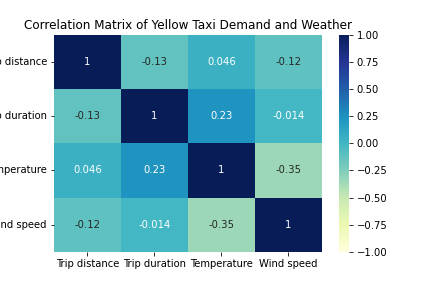
\includegraphics[width=\textwidth]{plots/yellow weather.png}
         \subfloat{(a) Yellow Taxi}
     \end{minipage}
     \hfill
     \begin{minipage}[b]{0.495\textwidth}
         \centering
         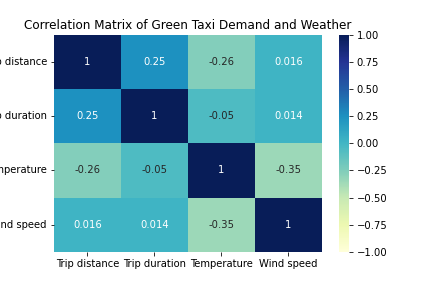
\includegraphics[width=\textwidth]{plots/green weather.png}
         \subfloat{(b) Green Taxi}
     \end{minipage}
     \hfill
     \caption{Correlation Matrix of Taxi Demands and Weather}
\end{figure}

\subsubsection{Pick up location}
This feature is used for the purpose of geospatial visualization as this report mainly emphasizes the relationship of weather and trip distance in NYC as a whole regardless of the pickup location. Figure 3 displays the mean distance across NYC based on the pick up location.

\begin{figure}[ht]
     \centering
     \begin{minipage}[b]{0.49\textwidth}
         \centering
         \includegraphics[width=\textwidth]{plots/yellow trip.png}
         \subfloat{(a) Yellow Taxi}
     \end{minipage}
     \hfill
     \begin{minipage}[b]{0.495\textwidth}
         \centering
         \includegraphics[width=\textwidth]{plots/green trip.png}
         \subfloat{(b) Green Taxi}
     \end{minipage}
     \hfill
     \caption{Geospatial Visualization of Mean Taxi Ride Distance}
\end{figure}

\subsubsection{Mean distance}
The mean distance of hourly taxi trips per day was generated for both taxis. It is hypothesized that if there was a shorter mean distance during that time, it would be due to the impact of drastic weather. From the correlation matrix in Figure 2, yellow taxi's mean trip distance shows a weak negative correlation to wind speed and a very weak positive correlation to temperature. On the other hand, the green taxi's mean trip distance shows a weak negative correlation to temperature to temperature and a very weak positive correlation to wind speed.


\subsubsection{Weather}
\begin{figure}[ht]
     \centering
     \begin{minipage}[b]{0.495\textwidth}
         \centering
         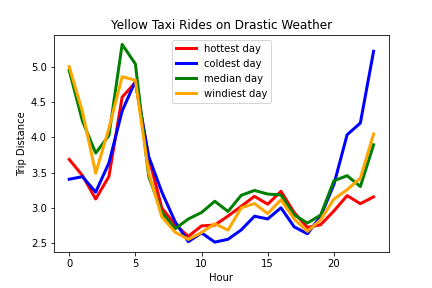
\includegraphics[width=\textwidth]{plots/yellow time series.png}
         \subfloat{(a) Yellow Taxi}
     \end{minipage}
     \hfill
     \begin{minipage}[b]{0.495\textwidth}
         \centering
         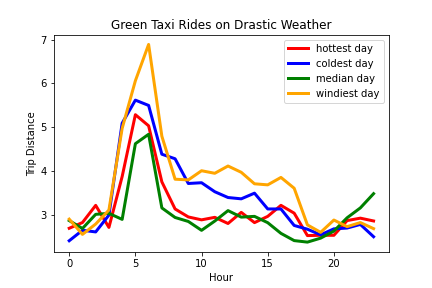
\includegraphics[width=\textwidth]{plots/green time series.png}
         \subfloat{(b) Green Taxi}
     \end{minipage}
     \hfill
     \caption{Time Series Analysis during Drastic Weathers in NYC}
\end{figure}
The weather data consists of temperature and wind speed to find the coldest day, hottest day, and windiest day in NYC during the first half of 2019. This is to be sure regarding how drastic weathers may effect the behavior in which people decide to take a taxi even if their destination is close. Figure 4 shows the trip distance of both taxis during days with drastic weather and regular days.


From Figure 4, it could be observed that both taxis show a similar trend where generally a spike in mean trip distance can be observed at approximately 5 A.M. For yellow taxis, the general day demonstrates an overall higher mean trip distance compared to the days with drastic weather. However, another significant increase can be observed after 8 P.M. for the coldest day. As for green taxis, the average day shows overall lower mean trip distance whereas the windiest day displays the highest overall mean trip distance. Based on the analysis of Figure 2 and Figure 3, it would be safe to assume that despite the low correlation of the variables, this does not guarantee the fact that relationships between the variables don't exist. Therefore we would compare two models: Linear regression and Poisson regression. 

\section{Modelling}
This section will discuss the models used for this analysis and then compare the results for both models.
\subsection{Linear Regression}
The linear regression model is used in this report to predict the values of the mean trip distance per hour of the day, which is done by estimating the coefficient of the linear equation. Given the input of the full first half of 2019 has been split into a 90-10 training and testing data, then testing data was then evaluated to provide the regression output of the mean trip distance per hour of the day. The accuracy metrics such as mean absolute error (MAE (1)), mean squared error (MSE (2)), and R-squared (3) are also acquired in order to evaluate the prediction error rates and model performance in the regression analysis with formulas below.

\begin{equation}
  \centering
  MAE = \frac{1}{N}\sum_{i=1}^{N}|y_i-\hat{y}|  
\end{equation}

\begin{equation}
  \centering
  MSE = \frac{1}{N}\sum_{i=1}^{N}(y_i-\hat{y})^2
\end{equation}

\begin{equation}
  \centering
  R^2 = 1 - \frac{\sum_(y_i-\hat{y})^2}{\sum_(y_i-\bar{y})^2}
\end{equation}

\subsection{Poisson Regression}
Poisson regression is equipped to predict the dependent variable (in this case the mean trip distance) as it contains a count data. The Poisson regression assumes that the response variable has a Poisson distribution and that the expected model can be calculated by a linear combination of the unknown parameters. This model is suitable as it can equip count data on the numerical taxi and weather dataset.

Accuracy metric results are the same as those from linear regression: MAE, MSE, and R-squared values in order to predict the competence of this model for predicting taxi consumer behavior impacted by weather.

\subsubsection{Prediction and Error Analysis}
As recalled in Section 1, this report assumes the perspective of a taxi company with the objective of predicting the demand of taxis around NYC regardless of distance during drastic weathers. Predictions are made by evaluating the test set.
\begin{table}[h!]
\centering
\begin{tabular}{||c c c c||} 
 \hline
 Taxi & Mean Absolute Error & Mean Squared Error & R-squared \\ [0.5ex] 
 \hline\hline
 Yellow & 0.54 & 0.48 & -0.01\\ 
 \hline
 Green & 0.61 & 0.82 & 0.09\\
 \hline
\end{tabular}
\caption{Linear Regression Model Accuracy Results}
\label{table:1}
\end{table}

The results for the linear regression model can be seen in Table 1, which shows a high overall MAE and MSE for both yellow and green taxis as well as a poor R-squared value for both taxis. 

\begin{table}[h!]
\centering
\begin{tabular}{||c c c c||} 
 \hline
 Taxi & Mean Absolute Error & Mean Squared Error & R-squared \\ [0.5ex] 
 \hline\hline
 Yellow & 0.51 & 0.49 & -0.01\\ 
 \hline
 Green & 0.62 & 0.78 & 0.09\\
 \hline
\end{tabular}
\caption{Poisson Regression Model Accuracy Results}
\label{table:2}
\end{table}

The Poisson regression model show similar results as a high overall MAE and MSE for both yellow and green taxis as well as a poor R-squared value for both taxis can be observed in Table 2.



\section{Recommendations}
As observed in Table 1 and Table 2, regression models are not suitable for predicting taxi demand during drastic weather. Limitations include grouping and averaging the variables per hour of the day instead of looking at the individual taxi rides to eliminate the overfitting or underfitting of data. Another recommendation would be to use a non-linear model as Figure 2 have indicated the weak linear relationships between trip distance and weather. Figure 4 suggested that factors such as time of the day may also be a factor in effecting the taxi demand, highlighting the importance that future studies must take into account the work and busy hours of NYC. 

The investigation in this report is limited by the amount of features used, suggesting that other features in the weather data should also be equipped to discover an underlying variable. Another suggestion regarding features would be to equip a neural network model to predict the taxi demand based on multiple features outside of weather, as there are countless of features that could actually impact taxi demand other than weather. Figure 3 has also talked about pick up location, however the variable isn't deemed significant. Future studies may analyze further the effect of taxi location on taxi demand while predicting future data.

Taxi companies must therefore conduct further research in order to be able to improve their products' demands. 

\section{Conclusion}
In conclusion, regression models aren't suitable for predicting taxi demand based on solely temperature and wind speed in weather. It would be recommended to use a neural network model to find out underlying features that may or may not impact taxi demand. Locations should also be pin pointed as the analysis of NYC as a whole may be too broad. Based on the results, there isn't enough evidence that there is a relationship between an increase in taxi demand regardless of trip distance and weather.


\clearpage

% BEGIN REFERENCES SECTION
\printbibliography
\end{document}